\documentclass[11pt,english]{article}

%%%%%%%%%%%%%%%%%%%%%%%%%%%%%%%%%%%%%%%%%%%%%%%%%%%%%%%%%%%
% Packages
%%%%%%%%%%%%%%%%%%%%%%%%%%%%%%%%%%%%%%%%%%%%%%%%%%%%%%%%%%%

% paper size & margins
\usepackage{fullpage}
\usepackage[showframe=false,margin=1in]{geometry}
\parindent=0pt

% font management
\usepackage{relsize}
\usepackage[T1]{fontenc} % for properly hyphenating words with accented chars
\usepackage[latin1]{inputenc}
\usepackage{babel}

% math
\usepackage{amsmath}
\usepackage{amsthm, amssymb}
\usepackage{textcomp}
\usepackage{stmaryrd}
\usepackage{upgreek}
\usepackage{bm}
\usepackage[linesnumbered,ruled,vlined]{algorithm2e}

% assorted
\usepackage{url}
\usepackage{breakurl}
\usepackage{xspace}
\usepackage{comment}
\usepackage{color}
\usepackage{afterpage}
\usepackage{graphicx}
\usepackage{hyperref}
\usepackage{pdfpages}
\usepackage{subcaption}

%%%%%%%%%%%%%%%%%%%%%%%%%%%%%%%%%%%%%%%%%%%%%%%%%%%%%%%%%%%
% Shortcuts
%%%%%%%%%%%%%%%%%%%%%%%%%%%%%%%%%%%%%%%%%%%%%%%%%%%%%%%%%%%
\newcommand{\hide}[1]{}

%%%%%%%%%%%%%%%%%%%%%%%%%%%%%%%%%%%%%%%%%%%%%%%%%%%%%%%%%%%
% Title / Author
%%%%%%%%%%%%%%%%%%%%%%%%%%%%%%%%%%%%%%%%%%%%%%%%%%%%%%%%%%%
\begin{document}

\title{CS7643: Deep Learning \\
Fall 2019\\ HW1 Solutions}
\author{Nicolas \textsc{Six}}
\maketitle


%%%%%%%%%%%%%%%%%%%%%%%%%%%%%%%%%%%%%%%%%%%%%%%%%%%%%%%%%%%
% Body
%%%%%%%%%%%%%%%%%%%%%%%%%%%%%%%%%%%%%%%%%%%%%%%%%%%%%%%%%%%

    \section{Gradient Descent}
    \subsection{Minimisation of $\vec{w^*}$}
    
If this function has a minimum, it has to be when its partial derivative regarding to $\vec{w}$ is null.
In addition, as the this function is convex, so admit only one point where $\vec{w}$ is null, and so only one extrema.
As this function is clearly unbounded from above this extrema is the global minimum.

\begin{align*}
    \frac{\partial \left( f\left( \vec{w^{(t)}} \right) +
                           \left< \vec{w} - \vec{w^{(t)}}, \nabla f\left( \vec{w^{(t)}} \right) \right>
                           + \frac{\lambda}{2} \left\| \vec{w} - \vec{w^{(t)}} \right\|^2 \right)
    }{
        \partial \vec{w}
    }
    &= 0 \\
    \Leftrightarrow
    \frac{\partial \left(
                           \left< \vec{w}, \nabla f\left( \vec{w^{(t)}} \right) \right> \right) }
    {\partial \vec{w}} +
    \frac{\partial \left( \frac{\lambda}{2} \left< \vec{w} - \vec{w^{(t)}}, \vec{w} - \vec{w^{(t)}} \right> \right) }
    {\partial \vec{w}}
    &= 0 \\
    \Leftrightarrow
    \left< \frac{\partial\vec{w}}{\partial\vec{w}}, \nabla f\left( \vec{w^{(t)}} \right) \right> +
    \lambda \left< \frac{\partial\vec{w}}{\partial\vec{w}}, \vec{w} - \vec{w^{(t)}} \right>
    &= 0 \\
    \Leftrightarrow
    \left< \frac{\partial\vec{w}}{\partial\vec{w}}, \nabla f\left( \vec{w^{(t)}} \right) + \lambda \left( \vec{w} - \vec{w^{(t)}} \right) \right>
    &= 0 \\
    \Leftrightarrow
    \nabla f\left( \vec{w^{(t)}} \right) + \lambda \left( \vec{w} - \vec{w^{(t)}} \right)
    &= \vec{0} \\
    \Leftrightarrow
    \vec{w}
    &= \vec{w^{(t)}} - \frac{1}{\lambda} \nabla f\left( \vec{w^{(t)}} \right) \\
\end{align*}

In conclusion we get the following:

\begin{align*}
    \vec{w^*} &= \vec{w^{(t)}} - \frac{1}{\lambda} \nabla f\left( \vec{w^{(t)}} \right) \\
    \eta &= \frac{1}{\lambda}
\end{align*}

This show us that under our current set of assumption, the gradient descent is leading us the the optimal solution.

\pagebreak

    \subsection{Lema proof}
    The optimal policy is $("go","go")$.
Lets name this policy $\pi^*$.
Now we can compute the value of each state following this policy.

\begin{align*}
    V^*(S_2) &= r(S_2, "go") \\
    &= 3
    V^*(S_1) &= r(S_1, "go") + \gamma V^*(S_2) \\
    &= -2 + 3 \gamma
\end{align*}




\pagebreak

    \subsection{Convergence rate}
    

\begin{align*}
    V^0 &= [0,0] \\
    V^1 &= [-1,3] \\
    V^2 &= [1,3] \\
    V^3 &= [1,3] \\
    V^* &= [1,3]
\end{align*}


\pagebreak

    \subsection{Convergence guarantee}
    
\paragraph{}
For this question we will suppose that $W$ is a diagonalizable matrix, which is implied by the fact that it's
eigenvalues are given in the subject.

With that in mind, we know that it exist a matrix $Q$ such as:

\[
    W^T = Q D Q^{-1}
\]

\paragraph{}
With $D$ being a diagonal matrix with tha eigenvalues of $W$ on the diagonal (and $Q$ the eigenvectors).

\paragraph{}
Using this we can easily rewrite the given equation as:
\begin{align*}
    h_t &= W^T h_{t-1} \\
        &= Q D Q^{-1} h_{t-1} \\
    h_t &= Q D^t Q^{-1} h_{0}
\end{align*}

\paragraph{}
It is trivial that raising a diagonal matrix to a power $t$ is equivalent to raise each of it's diagonal element to the
power $t$.
So depending on the value of the eigenvalues, raising the matrix $D$ to a high power will make the diagonal element
tend to zero (vanish) if they are smaller than one (in absolute value).
If they are bigger than one (in absolute value) they will diverge to infinity.
Or change signs / stay the same of they are $1$ or $-1$.

\paragraph{}
This matrix is then used to compute the output, $h_t$, but also in the backward pass to propagate the gradient.
Especially for the first inputs.
So the gradient could be multiplied by values that are either too big (exploding) or too small (vanishing).



\pagebreak

    \section{Automatic Differentiation}
    \subsection{Computation graph}
    
\begin{figure}
    \begin{center}
        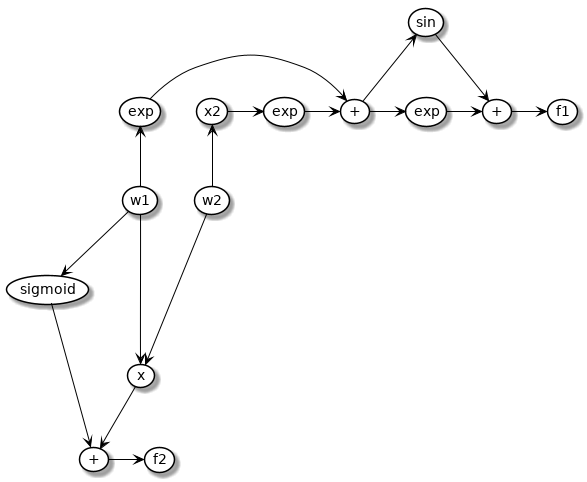
\includegraphics[width=0.9\linewidth]{../2_automatocDifferentiation/computation_graph.png}
        \caption{Computation graph for $\vec{f}$}
    \end{center}
\end{figure}

\pagebreak

    \subsection{Jacobian and numerical differentiation}
    With:
\begin{align*}
    f_1(1,2) &= 24521.662861313 \\
    f_2(1,2) &= 2.73105857863 \\
    f_1(1.01,2) &= 25200.8058793246 \\
    f_2(1.01,2) &= 2.75302014923886 \\
    f_1(1,2.01) &= 26411.9854338567 \\
    f_2(1,2.01) &= 2.74105857863
\end{align*}
We have:
\begin{align*}
    \frac{\partial \vec{f}}{\partial \vec{w}} &=
    \begin{bmatrix}
        \frac{f_1(1 + \Delta,2) - f_1(1,2)}{\Delta} & \frac{f_1(1,2 + \Delta) - f_1(1,2)}{\Delta} \\
        \frac{f_2(1 + \Delta,2) - f_2(1,2)}{\Delta} & \frac{f_2(1,2 + \Delta) - f_2(1,2)}{\Delta}
    \end{bmatrix} \\
    &=
    \begin{bmatrix}
        67914.3018011622 & 189032.25725437 \\
        2.19615706088527 & 0.999999999999979
    \end{bmatrix} \\
\end{align*}





\pagebreak

    \subsection{Forward mode auto-differentiation}
    

\begin{figure}[h!]
    \begin{center}
        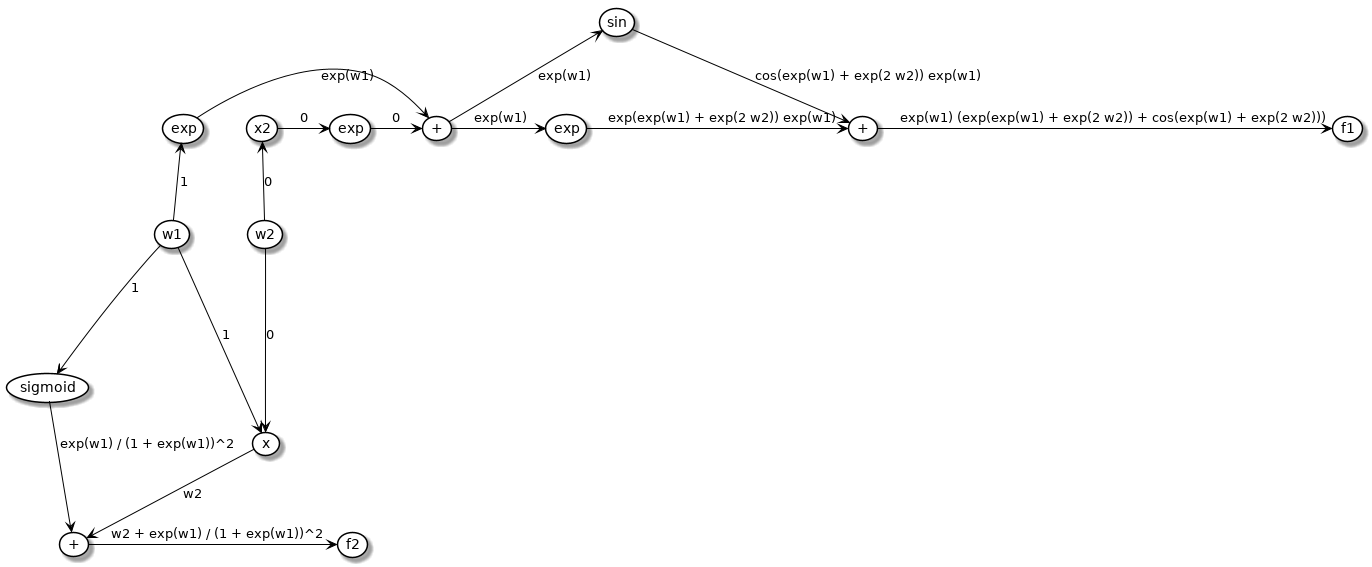
\includegraphics[width=.95\textwidth]{../2_automatocDifferentiation/computation_graph_forward_w1.png}
        \caption{Forward gradient decent on $\vec{f}$ for $w1$}
    \end{center}
\end{figure}

\begin{figure}[h!]
    \begin{center}
        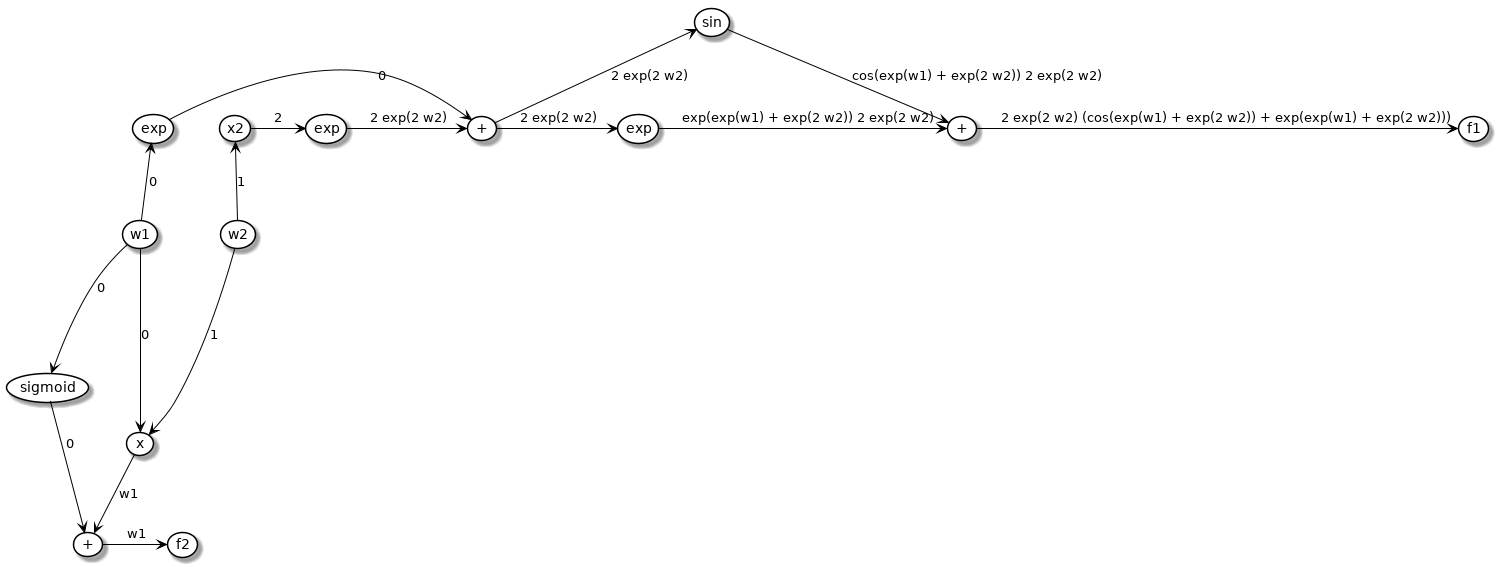
\includegraphics[width=.95\textwidth]{../2_automatocDifferentiation/computation_graph_forward_w2.png}
        \caption{Forward gradient decent on $\vec{f}$ for $w2$}
    \end{center}
\end{figure}

Which in a more mathematical format give us:

\[
    \frac{\partial \vec{f}}{\partial \vec{w}} =
    \begin{bmatrix}
        ( \cos(e^{w_1} + e^{2 w_2}) + e^{e^{w_1} + e^{2 w_2}} ) e^{w_1}   &   2 ( \cos(e^{w_1} + e^{2 w_2}) + e^{e^{w_1} + e^{2 w_2}} ) e^{2 w_2} \\
        \frac{e^{w_1}}{(1 + e^{w_1})^2} + w_2                             &   w_1
    \end{bmatrix}
\]



\pagebreak

    \subsection{Backward mode auto-differentiation}
    

\begin{figure}
    \begin{center}
        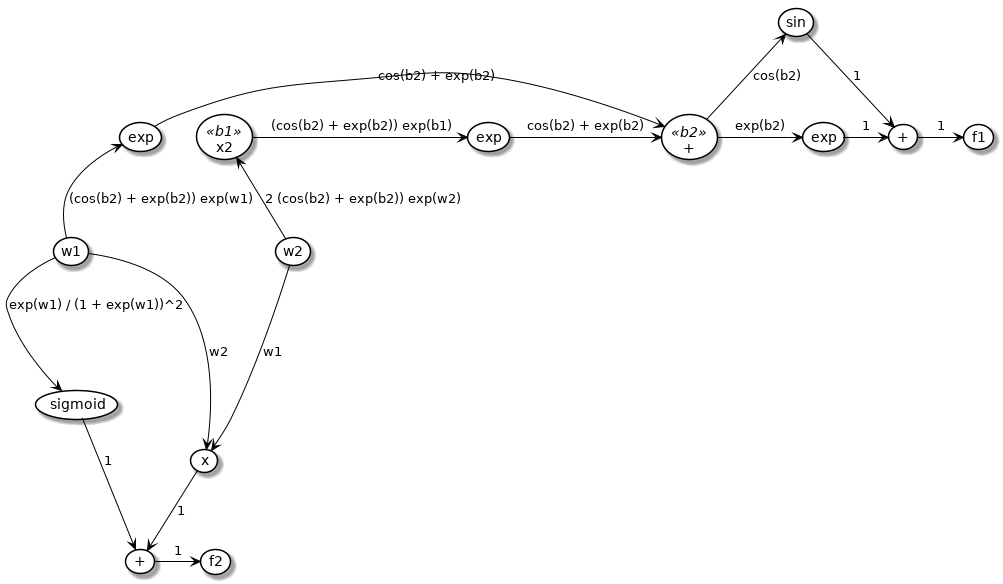
\includegraphics[width=\textwidth]{../2_automatocDifferentiation/computation_graph_backward.png}
        \caption{Backward gradient decent on $\vec{f}$}
    \end{center}
\end{figure}

Which in a more mathematical format give us:

\[
    \frac{\partial \vec{f}}{\partial \vec{w}} =
    \begin{bmatrix}
        ( \cos(e^{w_1} + e^{2 w_2}) + e^{e^{w_1} + e^{2 w_2}} ) e^{w_1}   &   2 ( \cos(e^{w_1} + e^{2 w_2}) + e^{e^{w_1} + e^{2 w_2}} ) e^{2 w_2} \\
        \frac{e^{w_1}}{(1 + e^{w_1})^2} + w_2                             &   w_1
    \end{bmatrix}
\]


\pagebreak

    \subsection{Automation}
    
\paragraph{}
Sure!


\pagebreak

    \section{Directed Acyclic Graphs (DAG)}
    \subsection{DAG imply topological ordering}
    
\paragraph{}
If $G$ is a DAG, then according to the lemma, at least one node has on input edges.
If we took such a node out of the graph as well as all the edges going from this node, the remaning graph would be a DAG
too (we only removed edges, we can't create cycle be removing edges).
We can now repeat the previous step on the newly created graph, until we got an empty graph.

The order in which we took the node out is a possible topological ordering.



\pagebreak

    \subsection{topological ordering imply DAG}
    \paragraph{}

If a graph has a topological ordering, then there is no edges going backward following this ordering.
Which mean that there is no cycle on the graph, as you can't go back to the place where you started to try creating your
graph, no matter where you try.
For the same reason there is either no edge in the graph or all the edges are directed.

So, if we have a graph with a valid topological ordering, we have a graph with directed edges and no cycle, a DAG.




\pagebreak

    \section{Implement and train a network on CIFAR-10}
    \subsection{cs231n}

    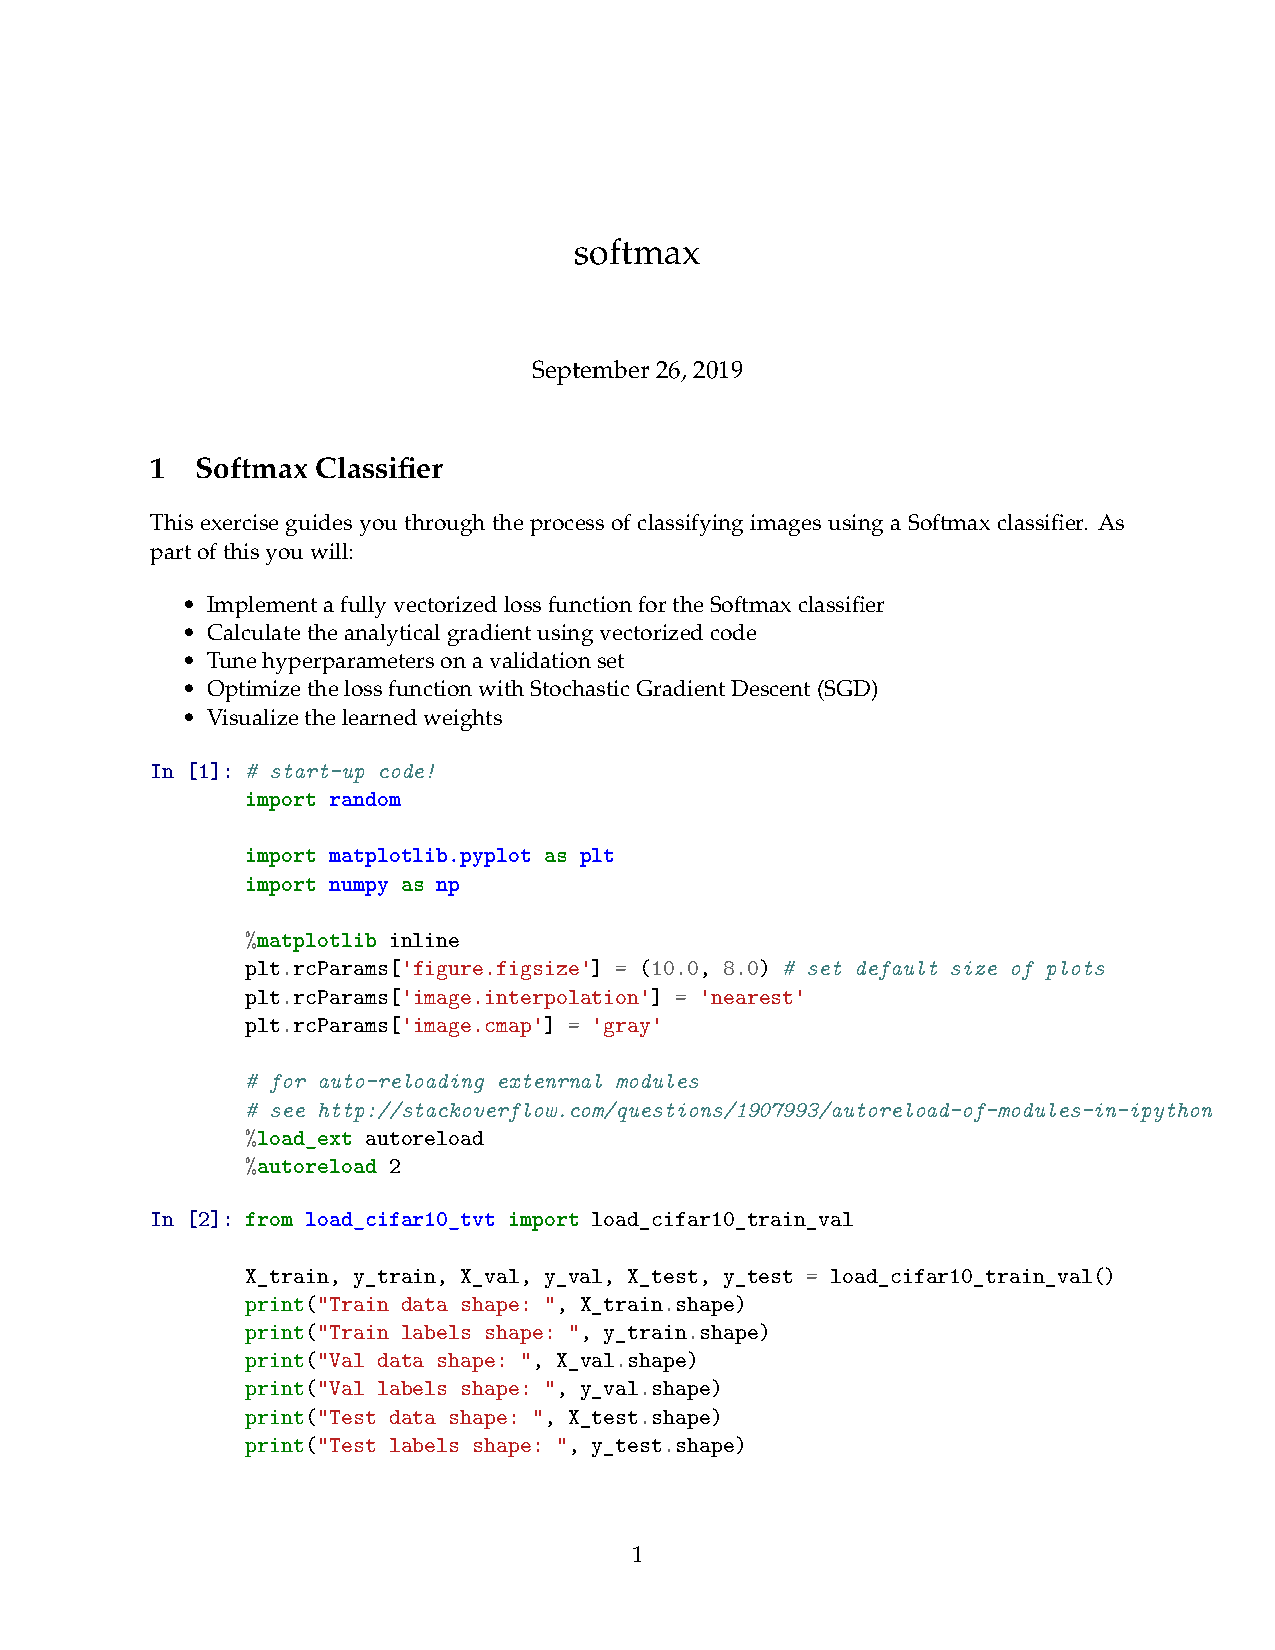
\includepdf[pages=-]{../code/assignment/1_cs231n/softmax.pdf}

    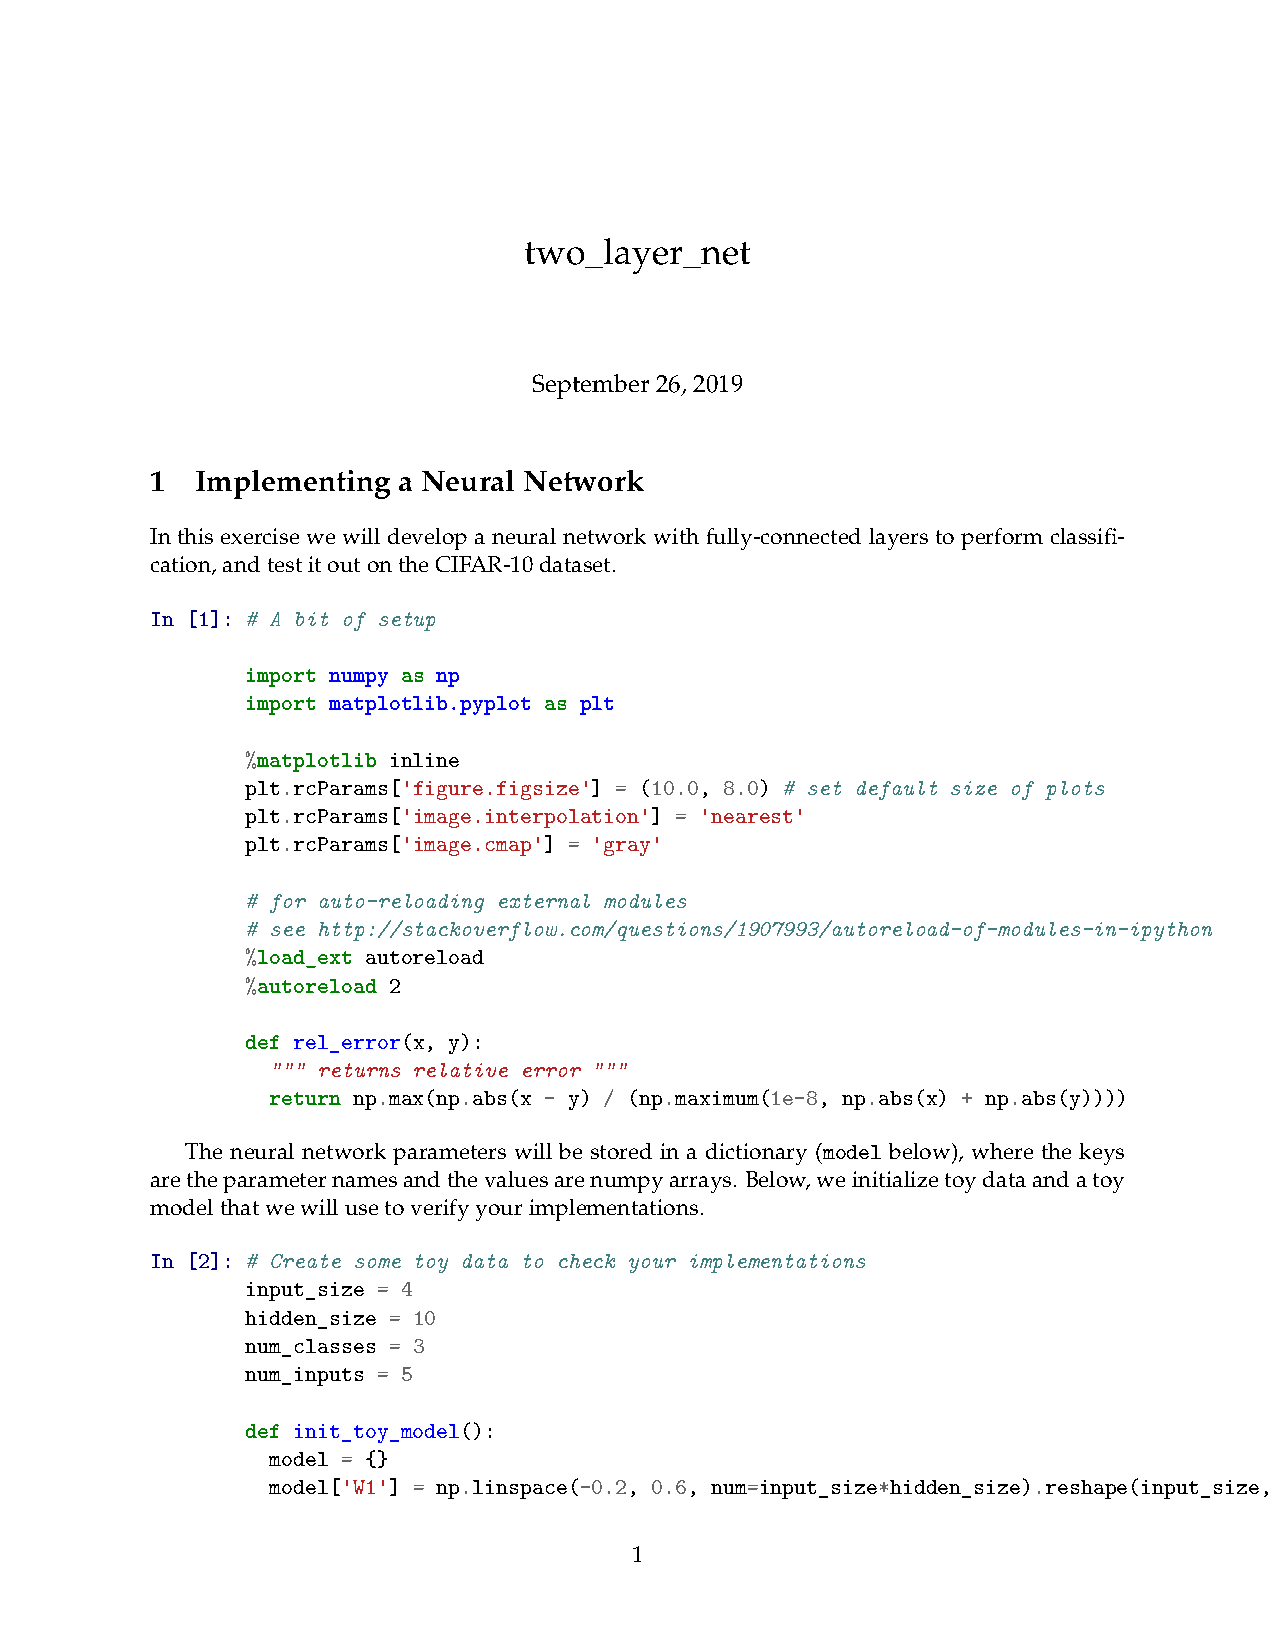
\includepdf[pages=-]{../code/assignment/1_cs231n/two_layer_net.pdf}

    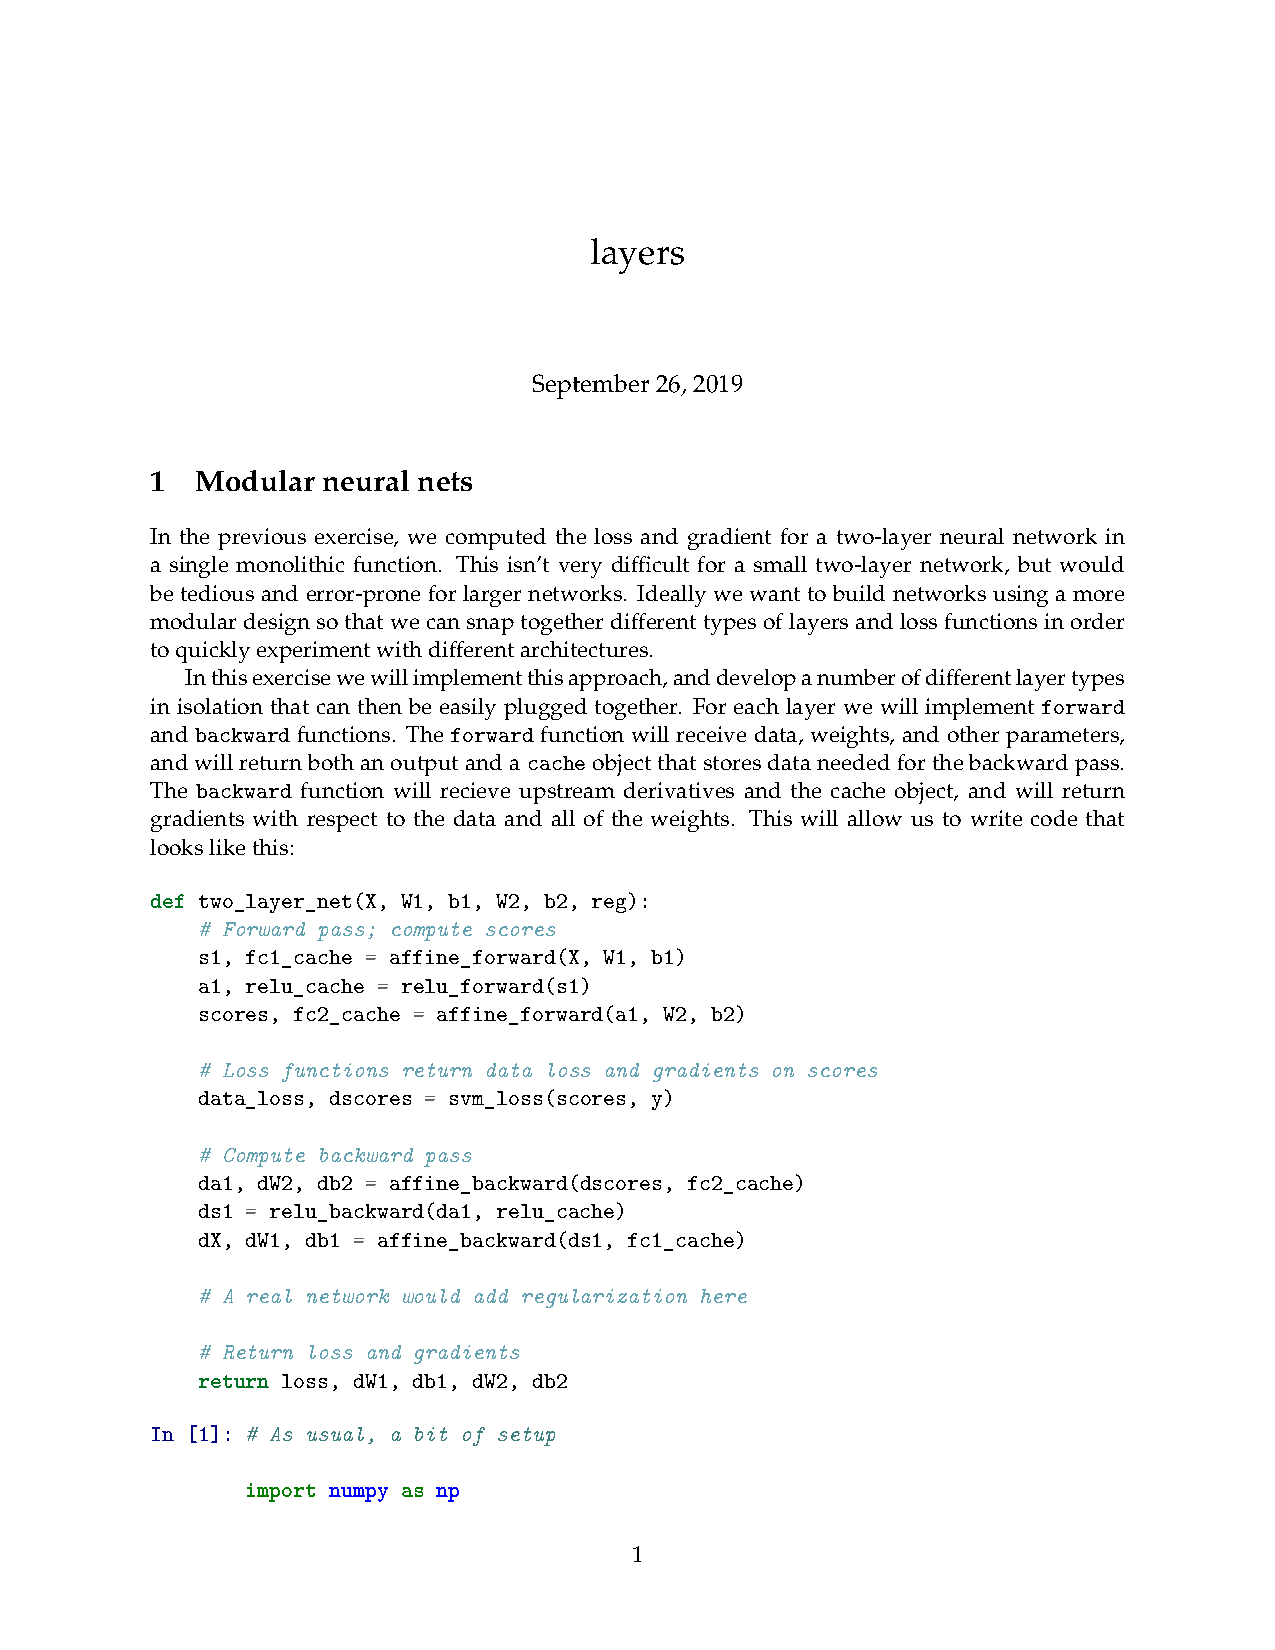
\includepdf[pages=-]{../code/assignment/1_cs231n/layers.pdf}

    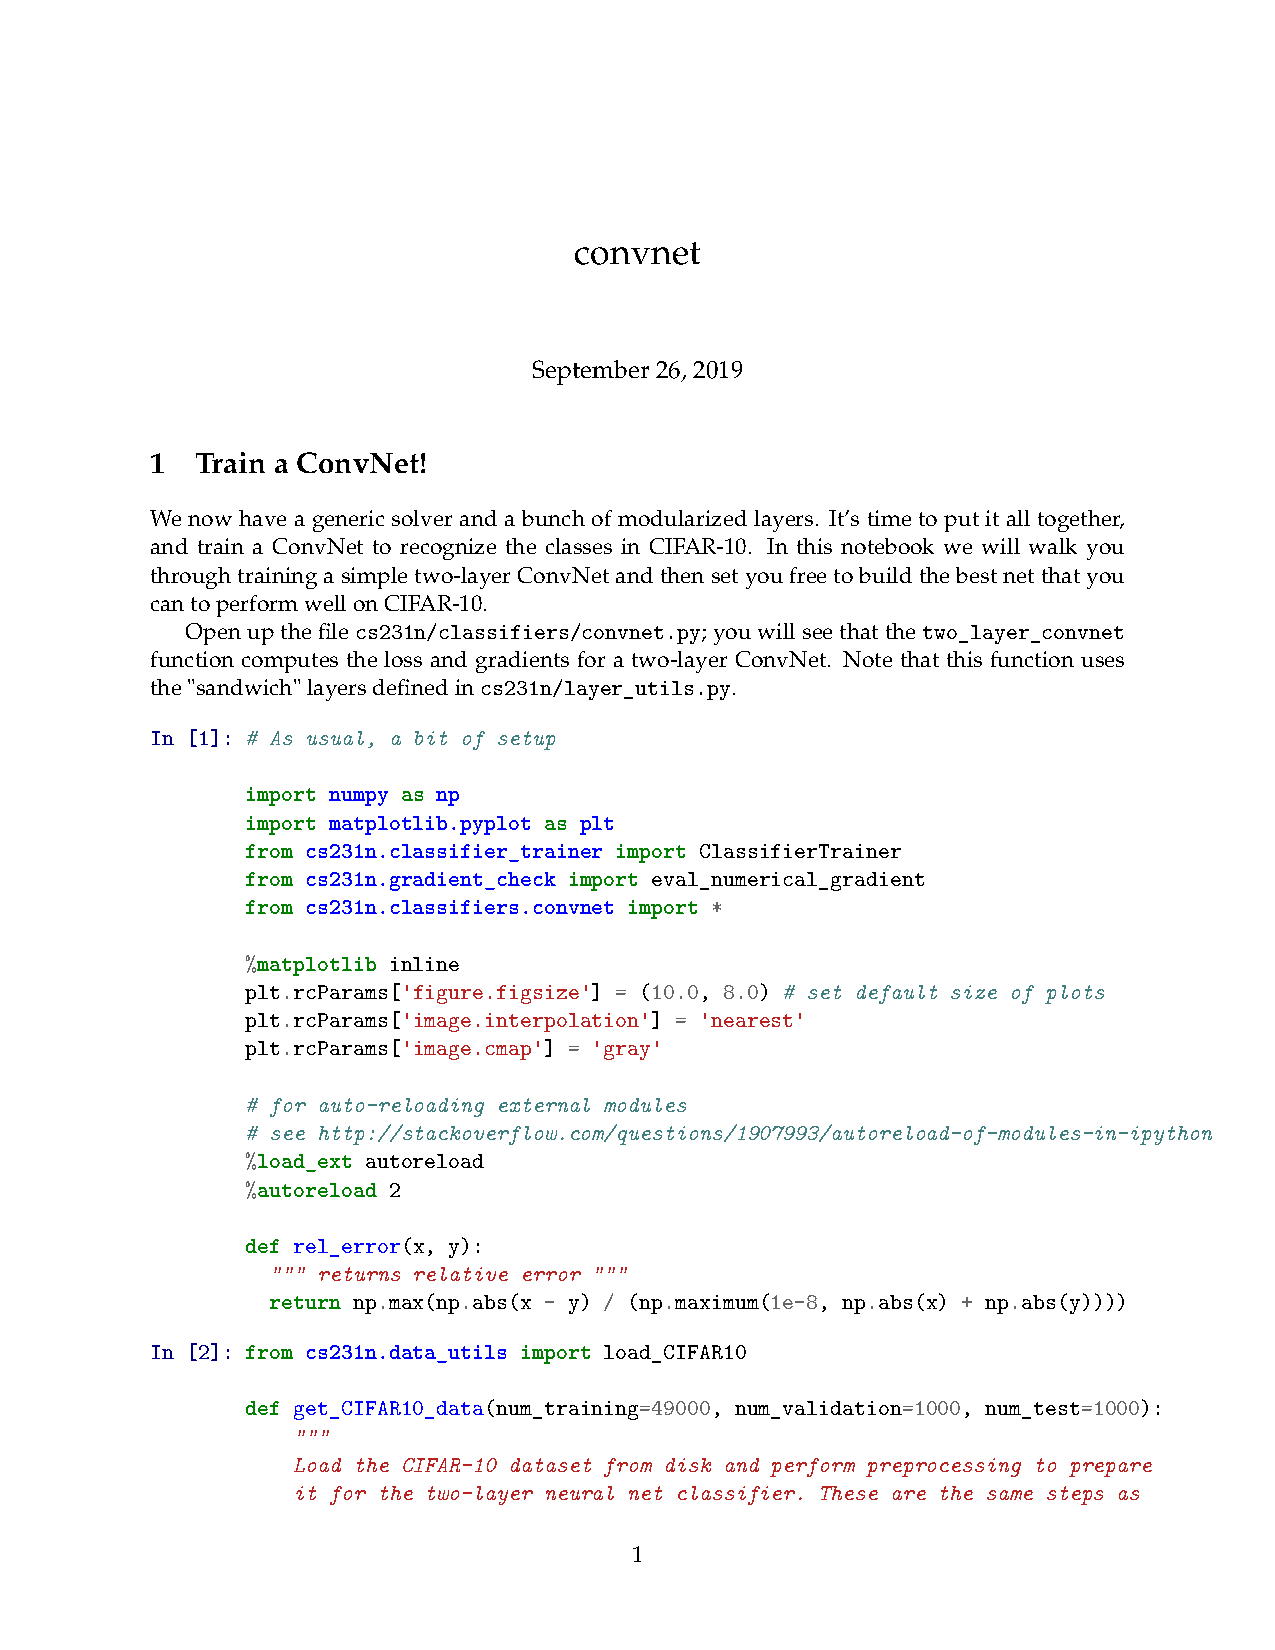
\includepdf[pages={1,2,3,4,5,6}]{../code/assignment/1_cs231n/convnet.pdf}

    \subsection{PyTorch}
    \subsubsection{Softmax}
    

\begin{figure}[h!]
  \begin{center}
    \begin{subfigure}[t]{0.49\linewidth}
      \centering
      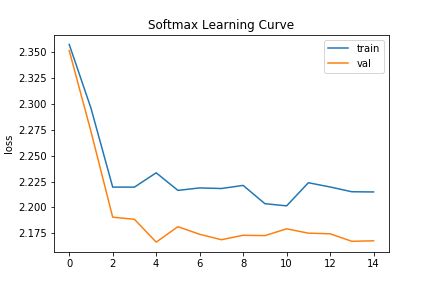
\includegraphics[width=\linewidth]{../code/assignment/2_pytorch/softmax_lossvstrain.png}
      \caption{Evolution of loss during training}
    \end{subfigure}
    \begin{subfigure}[t]{0.49\linewidth}
      \centering
      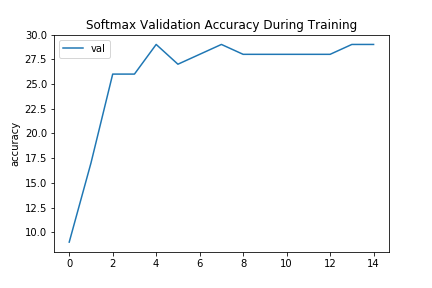
\includegraphics[width=\linewidth]{../code/assignment/2_pytorch/softmax_valaccuracy.png}
      \caption{Evolution of validation accuracy during training}
    \end{subfigure}
    \caption{Evolution of different indicators during training}
  \end{center}
\end{figure}

\begin{figure}[h!]
  \begin{center}
    \begin{subfigure}[t]{0.49\linewidth}
      \centering
      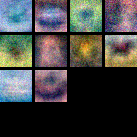
\includegraphics[width=\linewidth]{../code/assignment/2_pytorch/softmax_gridfilt.png}
        \caption{Filter of the trained softmax model displayed as a grid}
    \end{subfigure}
    \begin{subfigure}[t]{0.49\linewidth}
      \centering
      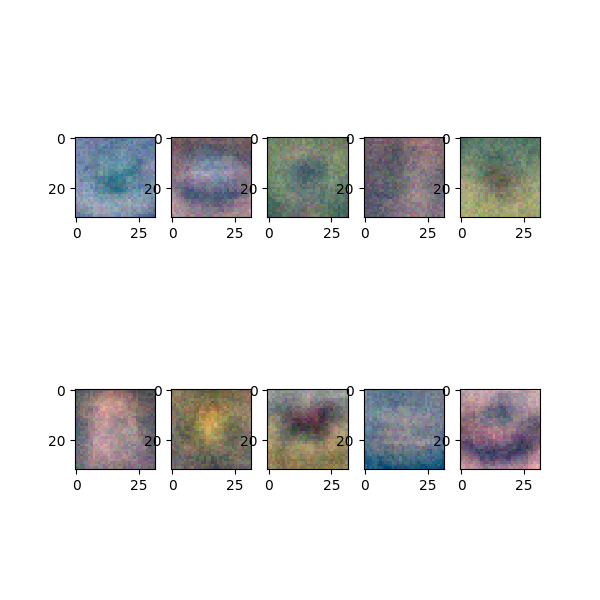
\includegraphics[width=\linewidth]{../code/assignment/2_pytorch/softmax_filt.png}
        \caption{Filter of the trained softmax model}
    \end{subfigure}
    \caption{Weights visualisation after training}
  \end{center}
\end{figure}


\pagebreak

    \subsubsection{Two layers NN}
    

\begin{figure}[h!]
  \begin{center}
    \begin{subfigure}[t]{0.49\linewidth}
      \centering
      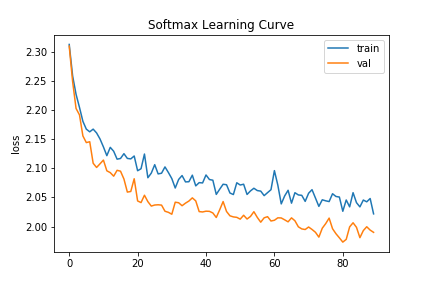
\includegraphics[width=\linewidth]{../code/assignment/2_pytorch/twolayernn_lossvstrain.png}
      \caption{Evolution of loss during training}
    \end{subfigure}
    \begin{subfigure}[t]{0.49\linewidth}
      \centering
      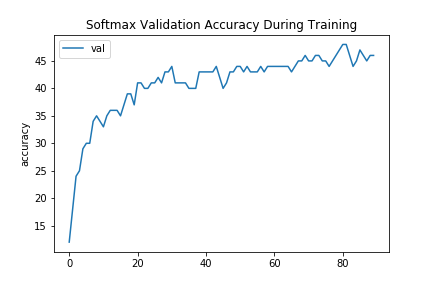
\includegraphics[width=\linewidth]{../code/assignment/2_pytorch/twolayernn_valaccuracy.png}
      \caption{Evolution of validation accuracy during training}
    \end{subfigure}
    \caption{Evolution of different indicators during training}
  \end{center}
\end{figure}

\begin{figure}[h!]
  \begin{center}
    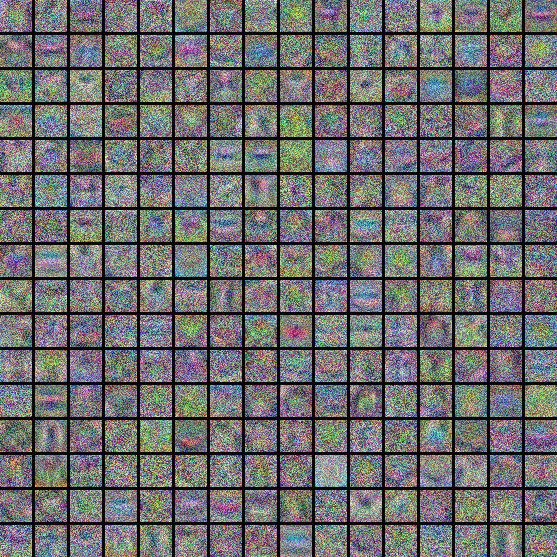
\includegraphics[width=.7\linewidth]{../code/assignment/2_pytorch/twolayernn_gridfilt.png}
    \caption{Filter of the trained softmax model displayed as a grid}
  \end{center}
\end{figure}


\pagebreak

    \subsubsection{Convnet}
    

\begin{figure}[h!]
  \begin{center}
    \begin{subfigure}[t]{0.49\linewidth}
      \centering
      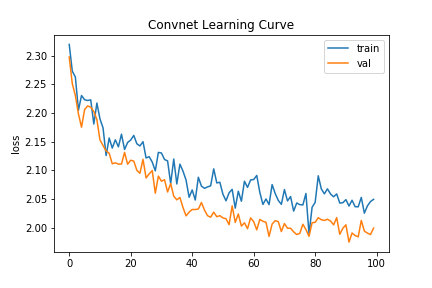
\includegraphics[width=\linewidth]{../code/assignment/2_pytorch/convnet_lossvstrain.png}
      \caption{Evolution of loss during training}
    \end{subfigure}
    \begin{subfigure}[t]{0.49\linewidth}
      \centering
      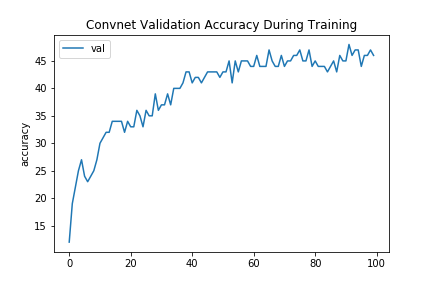
\includegraphics[width=\linewidth]{../code/assignment/2_pytorch/convnet_valaccuracy.png}
      \caption{Evolution of validation accuracy during training}
    \end{subfigure}
    \caption{Evolution of different indicators during training}
  \end{center}
\end{figure}

\begin{figure}[h!]
  \begin{center}
    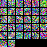
\includegraphics[width=.5\linewidth]{../code/assignment/2_pytorch/convnet_gridfilt.png}
    \caption{Filter of the trained softmax model displayed as a grid}
  \end{center}
\end{figure}


\pagebreak

    \subsubsection{Experimentation}
    

\begin{figure}[h!]
  \begin{center}
    \begin{subfigure}[t]{0.49\linewidth}
      \centering
      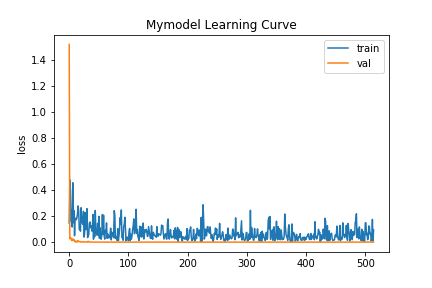
\includegraphics[width=\linewidth]{../code/assignment/2_pytorch/mymodel_lossvstrain.png}
      \caption{Evolution of loss during training}
    \end{subfigure}
    \begin{subfigure}[t]{0.49\linewidth}
      \centering
      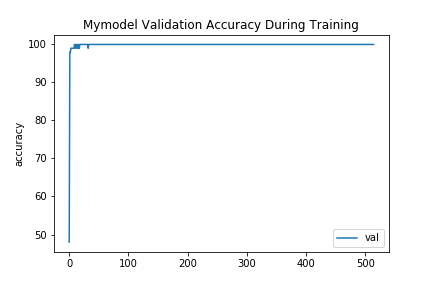
\includegraphics[width=\linewidth]{../code/assignment/2_pytorch/mymodel_valaccuracy.png}
      \caption{Evolution of validation accuracy during training}
    \end{subfigure}
    \caption{Evolution of different indicators during training}
  \end{center}
\end{figure}

%\section{Open challenge methodology}\label{open-challenge-methodology}

For this section I used the code and pre-trained weights from
https://github.com/quark0/darts I reimplemented the authors network on
the homework format, modified the \texttt{train.py} script to allow fine
tuning of existing weights and added data augmentation on the training
data. The pre-trained model being already trained on Cifar-10 using
architecture search, no much training were needed, one epoch was enough
for the network to take into account the difference on dataset loading.

I expect one or two percent accuracy can still be gained by re running
the architecture search and using more fine tuned data augmentation.

\begin{itemize}
\item
  Name: Nicolas Six
\item
  Email ID: nsix6 (nsix6@gatech.edu)
\item
  Best accuracy: 0.962 (EvalAI public set)
\end{itemize}




\end{document}
